\documentclass{itatnew}
%% !!!dolezite: ak pisete po slovensky alebo po cesky pouzite
%% \documentclass[slovensky]{itatnew}
%% \documentclass[cesky]{itatnew}

% Math shortcuts
\usepackage{amssymb}
\usepackage{algorithm}
\usepackage{algorithmic}
\newcommand{\xx}{\mathrm{\mathbf{x}}}
\newcommand{\yy}{\mathrm{\mathbf{y}}}
\newcommand{\XX}{\mathrm{\mathbf{X}}}
\newcommand{\CC}{\mathrm{\mathbf{C}}}
\newcommand{\ttheta}{\mathbf{\theta}}
\newcommand{\eell}{\boldsymbol\ell}
% \newcommand{\msf}[1]{\mathsf{\mathbf{#1}}}

\begin{document}

\title{Improving the Model Guided Sampling Optimization \\
  by Model Search and Slice Sampling}

\author{Lukáš Bajer\inst{1,2} \and Martin Holeňa\inst{2} \and Viktor Charypar \inst{3}}

\institute{Faculty of Mathematics and Physics, Charles University in Prague,\\
Malostranské nam. 25, 118 00 Prague 1, Czech Republic \\
\email{bajer@cs.cas.cz} \\
\and
Institute of Computer Science, Academy of Sciences of the Czech Republic,\\
Pod Vodárenskou věží 2, 182 07 Prague 8, Czech Republic \\
\email{martin@cs.cas.cz} \\
\and
Faculty of Nuclear Sciences and Physical Engineering, Czech Technical University in Prague, \\
Trojanova 13, 120 00 Prague 2, Czech Republic \\
\email{charyvik@fjfi.cvut.cz} }

\maketitle              % typeset the title of the contribution

\begin{abstract}
Model Guided Sampling Optimization (MGSO) was recently proposed as an alternative for Jones' Kriging-based EGO algorithm for optimization of expensive black-box functions. Instead of maximizing a chosen criterion (e.g., expected improvement), MGSO samples probability of improvement of the Gaussian process model forming multiple candidates -- a~whole population of suggested solutions. This paper further develops this algorithm using slice sampling method and continuous local optimization of the Gaussian process model.
\end{abstract}

\section{Introduction}
%
Optimization of expensive empirical functions forms an important topic in many engineering or natural-sciences areas. For such functions, it is often impossible to obtain any derivatives or information about smoothness; moreover, there is no mathematical expression nor algorithm to evaluate. Instead, some simulation or experiment has to be performed, and the measured value or result of such experiment is the value of the objective function being considered. Such functions are also called black-box functions. 
% Such empirical functions 
They are usually very expensive to evaluate; one evaluation may cost a lot of time and money to process.

Because of the absence of the derivatives, standard continuous first- or second-order derivative optimization methods cannot be used. Further, functions of this kind are usually characterized by a high number of local optima where simple algorithms can be trapped easily. Therefore, different derivative-free optimization methods for black-box functions (often called meta-heuristics) have been proposed. Even though these methods are slow and computationaly intensive, the cost of the evaluation of the empirical objective function is always much higher, and so it is cructial to decrease the number of function evaluations as much as possible.
% and the cost of these evaluations dominates the computational cost of the optimization algorithm.

Evolutionary algorithms constitute a broad family of meta-heuristics that are used for black-box optimization very frequently. Some of these algorithms and techniques are designed to minimize the number of objective function evaluations 
% for the optimization
All of the three following approaches use a model (of a different type in each case), which is built and updated within the optimization process.

\emph{Estimation of distribution algorithms} (EDAs) \cite{larranaga_estimation_2002} represent one such approach: EDAs iteratively estimate the probability distribution of selected candidate solutions (usually better than some threshold) and sample this distribution forming a new set of solutions for the next iteration. 

\emph{Surrogate modelling} is a technique of construction and usage of a regression model of the objective function~\cite{jin_comprehensive_2005}. The model (called surrogate model in this context) is then used to evaluate some of the candidate solutions instead of evaluating them with the original costly function.

Our method, \emph{Model Guided Sampling Optimization} (MGSO), takes inspiration from both these approaches. It uses a regression model of the objective function, which also provides an error estimate. However, instead of replacing the objective function with this model for some of the evaluations, it combines its prediction and the error estimate to get a probability of reaching a better solution in a given point. Similarly to EDAs, it then samples this pseudo-distribution\footnote{a function proportional to a probability distribution, it's value is given by the \emph{probability of improvement}, see Section~\ref{sec:sampling}} to obtain the next set of solution candidates.

The MGSO is similar to Jones' Efficient Global Optimization (EGO)~\cite{jones_efficient_1998}.
% like EGO, the MGSO uses a Gaussian process (GP, see~\cite{rasmussen_gaussian_2006} for reference), which provides a guide where to sample new candidate solutions in order to explore new solutions and exploit promising areas of the objective-function landscape.
Where EGO selects a \emph{single solution} maximizing a chosen criterion -- Expected Improvement (EI) or Probability of Improvement (PoI) -- the MGSO \emph{samples} the latter criterion. Hennig in his recent work~\cite{hennig_entropy_2012} examines more criteria in detail. 
% On the other hand, the MGSO samples GP model's latter criterion -- PoI.
% , producing a set of new points.
At the same time, the GP serves as a surrogate model of the objective function for small number of the solutions. In the second version of MGSO, presented in this paper, this smooth optimization is used in every generation of the optimization whereas the previous version employed model optimization only to improve the final optimum.
% During each iteration, MGSO samples the model's PoI forming a population of new candidate solutions, evaluates them and updates the GP model with the new gathered data.

This paper extends the previous brief introduction of MGSO~\cite{bajer_model_2013}. Instead of Gibbs' sampling, it uses slice sampling introduced by Neal~\cite{neal_slice_2003}. This enables computationally cheaper sampling and works even in higher dimensions where Gibbs' sampling fails. Further, the GP model is used as a surrogate model more often, which brings faster convergence in the number of function evaluations. The following section introduces methods used in the MGSO, Section~\ref{sec:mgso} describes the MGSO algorithm, and Section~\ref{sec:results} brings some preliminary results on the BBOB testing set~\cite{hansen_real_2009}.


\section{Involved Methods}

\subsection{Gaussian Processes}

Gaussian process~\cite{rasmussen_gaussian_2006} is a probabilistic model based on Gaussian distributions. This type of model was chosen because it predicts the function value in a new point in the form of univariate Gaussian distribution: the mean and the standard deviation of the function value are provided. Through the predicted mean, the GP can serve as a surrogate model, and the standard deviation is an estimate of uncertainty of the prediction in a specified point.

The GP is specified by mean and covariance functions and relatively small number of covariance function's hyper-parameters. The hyper-parameters are fitted by the maximum-likelihood method.

Let $\XX_N = \{\xx_i \ | \ \xx_i \in \mathbb{R}^{D}\}_{i=1}^{N}$ be a set of $N$ training $D$-dimensional data points with known dependent-variable values $\yy_N = \{y_i\}_{i=1}^{N}$ and $f(\xx)$ be an unknown function being modelled for which $f(\xx_i) = y_i$ for all $i \in \{1,\ldots,N\}$. The GP model imposes a probabilistic model on the data: the vector of known function values $\yy_N$ is considered to be a sample of a $N$-dimensional multivariate Gaussian distribution with probability density $p(\yy_N \, | \, \XX_N)$. If we take into consideration a new data point $(\xx_{N+1}, y_{N+1})$, the new probability density is
\begin{equation}
p(\yy_{N+1} \, | \, \XX_{N+1}) = \frac { \exp(-\frac{1}{2} \yy^\top_{N+1} \CC^{-1}_{N+1} \yy_{N+1}) } { \sqrt{(2\pi)^{N+1} \det(\CC_{N+1})} }
\end{equation}
where $\CC_{N+1}$ is the covariance matrix of the Gaussian distribution (for which mean is usually set to constant zero) and 
$\yy_{N+1} = \{y_1,\ldots,y_N, y_{N+1}\}$ (see \cite{buche_accelerating_2005} for details). This covariance can be written as
\begin{equation}
\CC_{N+1} = \left( \begin{array}{cc} \CC_N & \mathbf{k} \\ \mathbf{k}^\top & \kappa \end{array} \right)
\end{equation}
where $\CC_N$ is the covariance of the Gaussian distribution given the $N$ training data points, $\mathbf{k}$ is a vector of covariances between the new point and training data, and $\kappa$ is the variance of the new point itself.

Predictions in Gaussian processes are made using Bayesian inference. Since the inverse $\CC^{-1}_{N+1}$ of the extended covariance matrix can be expressed using inverse of the training covariance $\CC^{-1}_N$ and $\yy_N$ is known, the density of the distribution in a new point simplifies to a univariate Gaussian with the density
\begin{equation}
p(y_{N+1} \, | \, \XX_{N+1}, \yy_N) \ \varpropto \ \exp \left( -\frac{1}{2} \frac {(y_{N+1} - \hat{y}_{N+1})^2} {s^2_{y_{N+1}}} \right)
\label{univariate-density}
\end{equation}
with the mean and variance given by
\begin{eqnarray}
\hat{y}_{N+1} & = & \mathbf{k}^\top \CC^{-1}_N \yy_N, \\
s^2_{y_{N+1}} & = & \kappa - \mathbf{k}^\top \CC^{-1}_N \mathbf{k}.
\end{eqnarray}
Further details can be found in \cite{buche_accelerating_2005}.

The covariance $\CC_N$ plays a crucial role in these equations. It is defined by the covariance-function matrix $\mathbf{K}$ and signal noise $\sigma$ as
\begin{equation}
  \CC_N = \mathbf{K}_N + \sigma \mathbf{I}_N
\end{equation}
where $\mathbf{I}$ is an identity matrix of order $N$. Gaussian processes use parametrized covariance functions $K$ describing prior assumptions on the shape of the modeled function. The covariance between the function values at two data points $\xx_i$ and $\xx_j$ is given by $K(\xx_i, \xx_j)$, which forms the $(i,j)$-th element of the matrix $\mathbf{K}_N$ as well. In our case, we used the most common squared-exponential function
\begin{equation}
K(\xx_i, \xx_j) = \theta \exp \left( -\frac{1}{2\ell^2} (\xx_i - \xx_j)^\top(\xx_i - \xx_j) \right), % + \theta_2
\end{equation}
which is suitable when the modelled function is rather smooth. The closer the points $\xx_i$ and $\xx_j$ are, the closer the covariance function value is to 1 and the stronger correlation between the function values $f(\xx_i)$ and $f(\xx_j)$ is. The signal variance $\theta$ scales this correlation,
% , $\theta_2$ rises the value from zero and $\theta_3$ means a white noise of the diagonal elements of the matrix.
and the parameter $\ell$ is the characteristic length-scale with which the distance of two considered data points is compared. Our choice of the covariance function was motivated by its simplicity and the possibility of finding the hyper-parameter values by the maximum-likelihood method. 


\subsection{Sampling}
\label{sec:sampling}

The core step of the MGSO algorithm is the sampling of the probability of improvement. This probability is, for a chosen threshold $T$ of the function value, directly given by the predicted mean $\hat{f}(\xx) = \hat{y}$ and the standard deviation $\hat{s}(\xx) = s_{y}$ of the GP model $\hat{f}$ in any point $\xx$ of the input space
\begin{equation}
  \mathrm{PoI}_T(\xx) = \mathrm{\Phi}\left( \frac{T - \hat{f}(\xx)}{\hat{s}(\xx)} \right) = \mathrm{P}(\hat{f}(\xx) \leqq T),
\end{equation}
which corresponds to the value of cumulative distribution function (CDF) of the Gaussian with density (\ref{univariate-density}) for the value of threshold $T$. Even though all the variables come from Gaussian distribution, $\mathrm{PoI}(\xx)$ is definitely not Gaussian-shaped since it depends on the threshold $T$ and the function being modeled $f$ -- a typical example of the landscape of $\textrm{PoI}(\xx)$ in two dimensions for the Rastrigin function is depicted in Fig.\,\ref{fig:poi}.
The dependency on the modeled function also causes a lack of analytical marginals, derivatives or conditional probability densities.

\begin{figure}
  \centering
  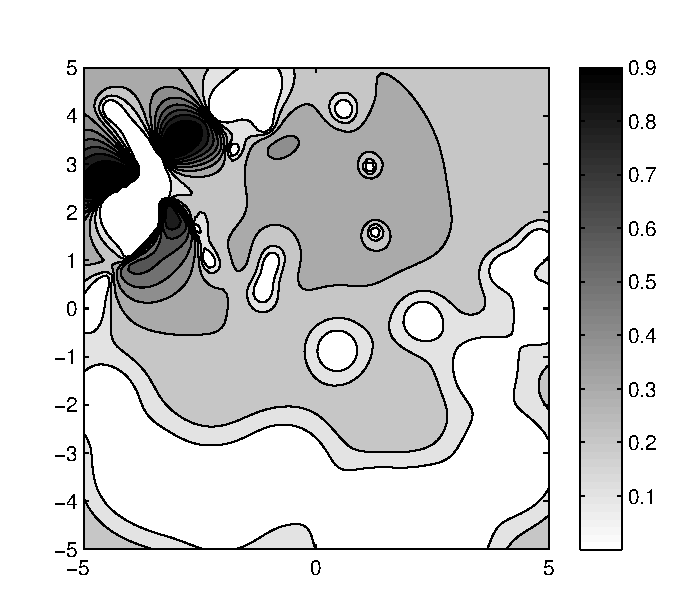
\includegraphics[width=0.75\linewidth]{poi_example_filled}
  {\small
  \caption{Probability of improvement. Rastrigin function in 2D, GP model built with 40 data points.
  \label{fig:poi}
  }
  }
\end{figure}

\paragraph{Gibbs' sampler.}

The first version of MGSO~\cite{bajer_model_2013} used Gibbs' sampler~\cite{geman_stochastic_1984}. The sampler starts at some point of the input space $\xx_s$. Further, it moves along each dimension to a new point $\xx'$: it cycles successively through each individual dimension $x_k$ of $\xx, k = 1,\ldots,D$ and samples from the conditional probability of $x_k$ given values of the remaining $x_{j \neq k}$: for $k=1,\ldots,D$
\begin{equation}
X_k \sim p(X_k \, | \, \{X_j = x_j, j \neq k)\}).
\end{equation}
As no analytical expression for these conditionals exists, piece-wise linear inverses of the empirical conditional CDF's $F^{-1}_k$ was used to transform samples from uniform distributions
\begin{displaymath}
u_k \sim U(0,1), \quad  x_k = F^{-1}_k(u_k).
\end{displaymath}
Linear interpolation between values of the empirical CDF was computed at the 20-points grid.

Even though evaluating GP model's mean $\hat{y} = \hat{f}(\xx)$ and standard deviation $\hat{s}(\xx)$ for 20 points requires only two calls of GP model prediction, the complexity of sampling rises quickly with the number of variables $D$, which causes that sampling in more than three dimensions becomes extremely slow.

\paragraph{Slice sampling.}

\begin{algorithm}[b]
\begin{algorithmic}[1]
{\small
\STATE \textbf{Input}: $f$ -- function proportional to the density \\
  \quad $\xx_0$ -- starting point, $\xx_0 \in \mathbb{R}^D$ \\
  \quad $\mathbf{w}$ -- scale estimates, $\mathbf{w} \in \mathbb{R}^D$ \\
  \quad $n$ -- required number of samples
\FOR {$k = 0,1,\ldots,n$}
  % \STATE \COMMENT{define the slice} \\
  \STATE $y \sim U(0, \, f(\xx_k))$  \hspace{\fill}  \COMMENT{height of the slice}
  % \STATE \COMMENT{random position of the hyper-rectangle} \\
  \STATE $\mathbf{u} \sim U(0,1)^D$ %  \hspace{\fill}  \COMMENT{random shift of hyper-rectangle}
  \STATE $\mathbf{L} \leftarrow \xx_k - \mathbf{w} \circ \mathbf{u}$  \hspace{\fill}  \COMMENT{randomly shifted lower bound} % \COMMENT{$\circ$ is entrywise product}
  \STATE $\mathbf{R} \leftarrow \mathbf{L} + \mathbf{w}$   \hspace{\fill}  \COMMENT{upper bound}
  % \STATE $\mathbf{L},\mathbf{R} \leftarrow$ lower/upper bounds of a hyper-rectangle $\mathbf{H}$ \\
  % \quad $\xx_k \in \mathbf{H}, \quad R_j - L_j = w_j \ \forall j = 1,\ldots,D$
  \WHILE {given number of tries has not been exceeded}
    \STATE $\mathbf{u} \sim U(0,1)^D$
    \STATE $\xx_{k+1} \leftarrow \mathbf{L} + \mathbf{u} \circ (\mathbf{R} - \mathbf{L})$ \hspace{\fill}  \COMMENT{$\xx_{k+1} \sim U(\mathbf{L},\mathbf{R})$}
    % \STATE $\xx_{k+1} \leftarrow$ random sample from the hyper-rectangle $[\mathbf{L}, \mathbf{R}]$
    \IF {$(y < f(\xx_{k+1}))$}
      \STATE accept $\xx_{k+1}$ and exit the \emph{while} loop
    \ENDIF
    \FOR {each dimension $j = 1,\ldots,D$}
      \IF {$(x^j_{k+1} < x^j_k)$}
      \STATE $L^j \leftarrow x^j_{k+1}$  \hspace{\fill}  \COMMENT{shrink the lower bound}
      \ELSE
      \STATE $R^j \leftarrow x^j_{k+1}$  \hspace{\fill}  \COMMENT{shrink the upper bound}
      \ENDIF
    \ENDFOR
  \ENDWHILE
\ENDFOR
\STATE \textbf{Output}: $\{\xx_1,\ldots,\xx_n\}$
}
\end{algorithmic}
\caption{Slice sampling~\cite{neal_slice_2003}}
\label{alg:slice}
\end{algorithm}

This novel kind of sampling, brought by Neal in 2003~\cite{neal_slice_2003}, is based on a simple and smart idea. Let $f$ be a function proportional to the density from which sampling is desired. It starts from a starting point $(\xx_0, f(\xx_0))$ where a uniform single-variable sample $y \sim U(0,f(\xx_0))$ is obtained. This value induces a subset $S=\{\xx \in \mathbb{R}^D \,|\, f(\xx) > y\}$, which is
% stepwise approximated by a hyper-rectangle and
uniformly sampled, forming a new point $\xx_1$. The sampler then starts again from this point $(\xx_1, f(\xx_1))$ and iteratively generates next samples.

The subspace $S$ is approximated with an axis-aligned hyper-rectangle $H$ of size $\mathbf{w} \in \mathbb{R}^D$, randomly positioned around the current point $\xx$ and successively shrinked if a point inside $H$ but outside $S$ is sampled. The parameter $\mathbf{w}$ is the only parameter of this method, which should not be much smaller than a typical size of the subset $S$. Larger values of $\mathbf{w}$ do not affect correctness and increase only moderatley the number of shrinking steps 13---19 in the pseudo-code Alg.\,\ref{alg:slice}. If the user-specified number of unsuccessful attempts of shrinking is exceeded, the slice sampling ends with an error, which possibly results in a lower number of individuals in the population during that MGSO generation.

Slice sampling has several advantages. First, it nicely scales with higher dimensionalities of the problem. Second, there is no need of conditional distributions as it is with Gibbs' sampler. Moreover, it does not require the density being normalized, which is the case of PoI. This kind of sampler is used in the second version of MGSO, described in this paper.


\section{Model Guided Sampling Optimization}
\label{sec:mgso}

As it was already mentioned, the MGSO algorithm for black-box optimization has many common aspects with Jones'~\cite{jones_efficient_1998} Efficient Global Optimization algorithm. Like some of the versions of EGO, it uses the probability of improvement $\mathrm{PoI}_T^{\mathsf{M}_i}(\xx)$ as a measure of how promising the specified point $\xx$ is for locating the optimum. This measure is given by a chosen threshold $T$ and the current knowledge of the function landscape
% saved in the current dataset $\mathsf{S}_i$ and
modelled by the current GP model $\mathsf{M}_i$. The main difference to EGO is that MGSO does not maximize this criterion, but it samples the PoI (which is proportional to a density) producing a whole population of individuals. 

After the initial (usually uniform random) sample of the input space, its evaluation and saving to the dataset $\mathsf{S}_0$, the MGSO algorithm proceeds as follows (see Alg.\,\ref{alg:mgso} for details; $\circ$ is a component-wise product of two vectors). First, a new GP model $\mathsf{M}_i$ is fitted to the current dataset $\mathsf{S}_i$. The model predictive distribution guides the further optimization: the model's PoI is sampled forming the new population.
The algorithm continues with evaluating the population, a new model is fitted to this augmented dataset and the process is repeated until a stopping condition (like the number of objective function evaluations) is met.

The second version of MGSO differs in two points. First, it uses the slice sampling instead of Gibb's sampler and second, a smooth model optimization (the step 6 in Alg.\,\ref{alg:mgso}) is added: the last individual in the population is obtained by continuous local optimization of the GP model. This search, which uses the GP as a surrogate model, speeds-up the optimization process especially in the final part of the algorithm's run. 

\begin{algorithm}[t]
\begin{algorithmic}[1]
{\small
  \STATE \textbf{Input}: $f$ -- objective function \\
      \quad $N', N$ -- sizes of the initial and standard population \\
      \quad $r$ -- the number of solutions for dataset restriction
  \STATE $\mathsf{S}_0 = \{(\xx_j, y_j)\}_{j=1}^{N'} \leftarrow$ generate $N'$ initial samples 
      and evaluate them % to get observed values $\{y_j\}_{j=1}^{N'}$ forming a dataset $\mathsf{S}_0 = \{(\xx_0, y_0)\}$
  \WHILE {no stopping condition is met, $i=1,2,\ldots$}
    \STATE $\mathsf{M}_i \leftarrow$ build a GP model and fit its hyper-parameters
        according to the dataset $\mathsf{S}_{i-1}$
    \STATE $\{\xx_j\}_{j=1}^{N}  \leftarrow$ sample the $\textrm{PoI}_T^{\mathsf{M}_i}(\xx)$ 
        forming $N$ new candidate solutions, optionally with different targets $T$
    \STATE $\xx_k \leftarrow$ find the minimum of the GP (by local continuous optimization) and replace the nearest solution from $\{\xx_j\}_{j=1}^{N}$ with it
    \STATE $\{y_j\}_{j=1}^N \leftarrow f(\{\xx_j\}_{j=1}^N)$  \hspace{\fill}  \COMMENT{evaluate the population} 
    \STATE $\mathsf{S}_i \leftarrow \mathsf{S}_{i-1} \cup \{(\xx_j, y_j)\}_{j=1}^N$  \hspace{\fill}  \COMMENT{augment the dataset} 
    \STATE $(\tilde{\xx}, \tilde{y}) \leftarrow \arg \min_{(\xx,y) \in \mathsf{S}_i} y$  \hspace{\fill}  \COMMENT{find the best solution in $\mathsf{S}_i$}
    \IF {any rescale condition is met} 
    \STATE restrict the dataset $\mathsf{S}_i$ to the bounding-box $[\mathbf{l}_i,\mathbf{u}_i]$ of the $r$ nearest solutions along the best solution $(\tilde{\xx},\tilde{y})$ and linearly transform $\mathsf{S}_i$ to $[-1, 1]^D$
    \ENDIF
  \ENDWHILE
  \STATE \textbf{Output}: the best found solution $(\tilde{\xx}, \tilde{y})$
}
\end{algorithmic}
\caption{MGSO (Model Guided Sampling Optimization)}
\label{alg:mgso}
\end{algorithm}


\subsection{Input Space Restriction}

To abstract from the search space scaling, MGSO works in an internal, linearly transformed coordinate system defined by mapping
\begin{equation}
\mathit{scale}:[\mathbf{l}, \mathbf{u}] \rightarrow [-1, 1]^D
\end{equation}
and the transformation can be updated during the optimization. Updating restricts the learning and sampling space to the neighborhood of the so-far optimum, which enables sampling in the situation when the PoI is non-zero only in a very small region. The lower and upper bounds $[\mathbf{l}_i, \mathbf{u}_i], \hspace{0.7em} \mathbf{l}_i,\mathbf{u}_i \in \mathbb{R}^D$ are determined as a bounding box of the $r$ nearest samples from the current optimum. 
The bounding box is expanded by 10\% in order not to have training points for the GP model on the boundaries of the training region.
The bounds $[\mathbf{l}_i, \mathbf{u}_i]$ can be updated each iteration~$i$, but, in practice, they are updated only several times during one optimization run.

The value $r$, the initial number of samples $N'$ and the population size $N$ are input parameters of MGSO. As this paper is still work-in-progress, no rigorous testing for the default values of these parameters has been performed yet. For the results presented in the next section, these values have been used: $r = 15 \cdot D$, $N = N' = 10 \cdot D$.

% the default is $r=15\cdot D$

  The slice sampling method enables us to sample multivariate distributions much faster. Slice sampling from Matlab Statistical toolbox was used, which implements shrinking-in of all dimensions. The sampler is extended by a validity-checking of the GP model -- the samples which, if added, result in ill-con\-di\-tion\-ed covariance matrix are rejected. These rejections start to occur in later phases of the algorithm run, which is a starting impulse for input space restriction and rescaling. Further, different thresholds $T$ for $\mathrm{PoI}_T^{\mathsf{M}_i}$ are tested if many ($N$ by default) such rejections arise.

\section{Experimental Results and Conclusion}
\label{sec:results}

Preliminary testing results from our Matlab implementation\footnote{the source code is freely available at \url{http://github.com/charypar/gpeda}} are comprised in this section. Because of large sampling time and low success rate of the Gibbs' sampler of the first MGSO in higher dimensions, speed of the optimization of the first and second version of MGSO is compared only in 2D testing cases. The second version of MGSO is further compared with the Covariance Matrix Adaptation Evolution Strategy (CMA-ES)~\cite{hansen_completely_2001} -- the state-of-the art in the field of continuous black-box optimization methods -- in 5D and 10D. The comparison of MGSO with Jones' EGO is forthcoming, but not included in this paper. More detailed evaluation of Gibbs' and slice sampling is placed in the first part of this section.

\subsection{Sampling}

The slice sampling has shown to be a noticeable improvement both in terms of the CPU time (for sampling and for the GP model evaluations) and the ability to provide enough samples from PoI. Illustrative results of the sampling CPU time and the number of GP model evaluations for two particular GP models in 2D and 5D are shown in Tab.\,\ref{tab:sampling} and sampling times and the numbers of successfully generated samples are depicted in Fig.\,\ref{fig:sampling}.

\begin{table}% [!bh]
\begin{center}
{\small
\caption{Comparison of Gibbs' and Slice sampling, results from 15 runs of sampling. Average CPU time and the number of evaluations of the GP model's PoI needed to generate 20/50 samples in 2D/5D. The differences of the CPU time per GP evaluation is mainly because of the batch evaluation of PoI for empir.\,CDF in Gibbs' sampler.}
\vspace{1ex}
\label{tab:sampling}
\begin{tabular}{l | c c c c}
\hline
            & Gibbs 2D  & slice 2D      & Gibbs 5D      & slice 5D \\
\hline
time [s]    & 1.85      & 1.11          & 42.41         & 17.56 \\
\# GP eval. & 2 402     & 246           & 20 087        & 2 909 \\
\hline
\end{tabular}
} % \small
% \vspace{2ex}
\end{center}
\end{table}

\begin{figure}
  \centering
  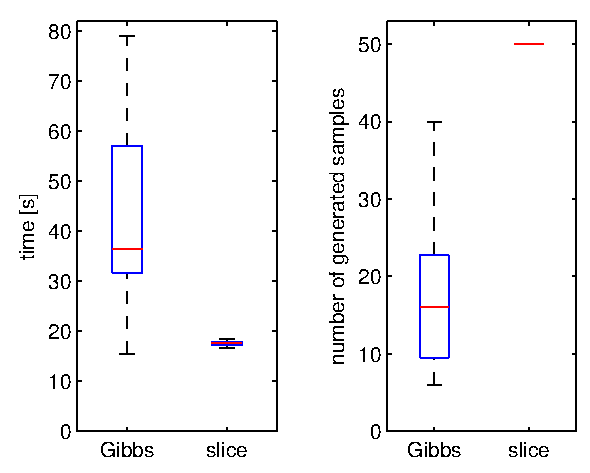
\includegraphics[width=0.7\linewidth]{sampling_time_popsize_5D}
  {\small
  \caption{Computational time and the number of successfully generated samples in 5D. Results from 15 independent runs with the same GP model/PoI.
  \label{fig:sampling}
  }
  }
\end{figure}

\subsection{BBOB Benchmark Functions Optimization}

The proposed MGSO has been tested on three different continuous benchmark functions from the BBOB testing set~\cite{hansen_real_2009}: sphere, Rosenbrock and Rastrigin functions. Although the previous version of the algorithm~\cite{bajer_model_2013} was practically able to optimize only two-dimensional versions of these functions, this paper provides results from 5D and 10D as well. The computational speed-up was caused mainly by the slice sampling method and partly also by the continuous model optimization step. % performed every iteration.

In two dimensions, the current version of the MGSO outperformed CMA-ES (considering budget 500 original evaluations) on both sphere and Rosenbrock functions, and it performs approximately equally well on Rastrigin function, see Fig.\,\ref{fig:optim_2D}. In terms of the CPU time for the whole optimization, the CMA-ES runs in several seconds while MGSO takes several or tens of minutes to process. But as we are concerned with expensive (usually empirical-function) optimization, we suppose the cost for the MGSO search being dominated by the time and money for the original evaluations.


\begin{figure}
  \centering
  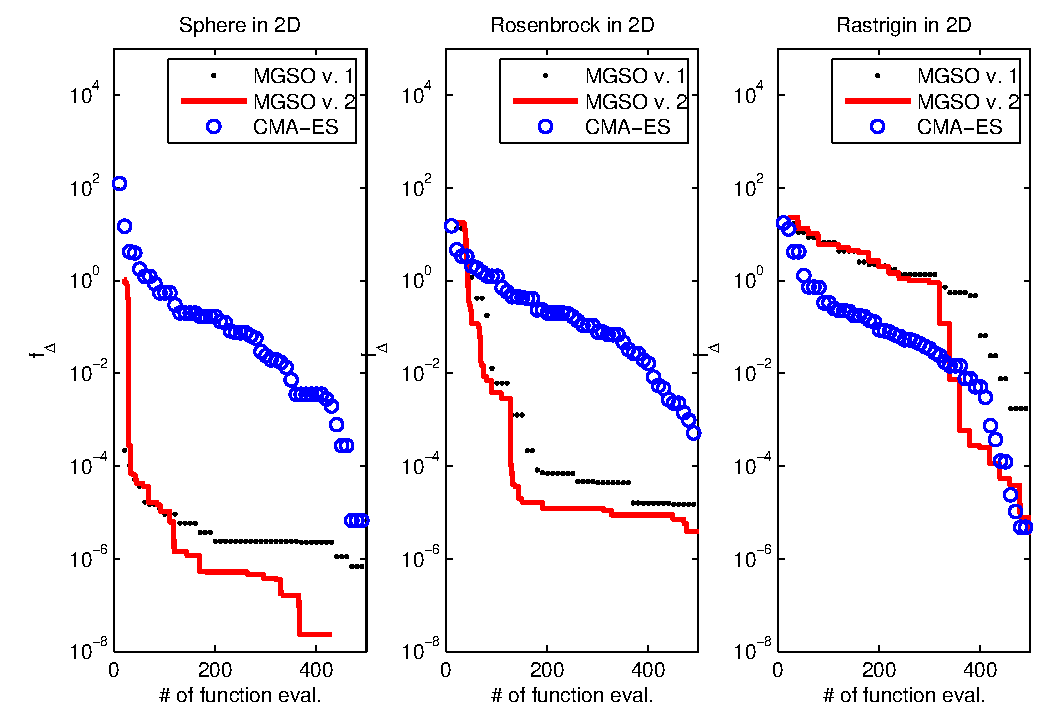
\includegraphics[width=\linewidth]{optim_2D_color}
  {\small
    \caption{2-D. Medians of the best found function values gathered from 15 independent runs. The First~\cite{bajer_model_2013} and the second version of MGSO are compared with CMA-ES.
  \label{fig:optim_2D}
  }
  }
\end{figure}

\begin{figure}
  \centering
  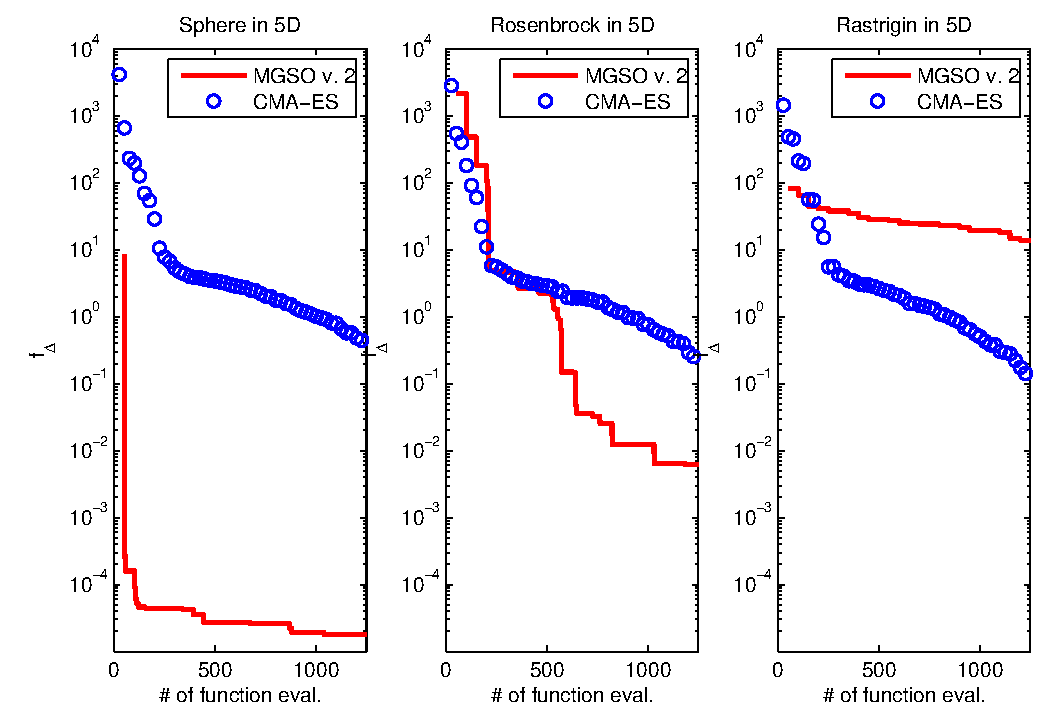
\includegraphics[width=\linewidth]{optim_5D_color}
  {\small
    \caption{5-D. Medians of the best found function values gathered from 15 runs. The second version of MGSO is compared to CMA-ES.
  \label{fig:optim_5D}
  }
  }
\end{figure}

\begin{figure}
  \centering
  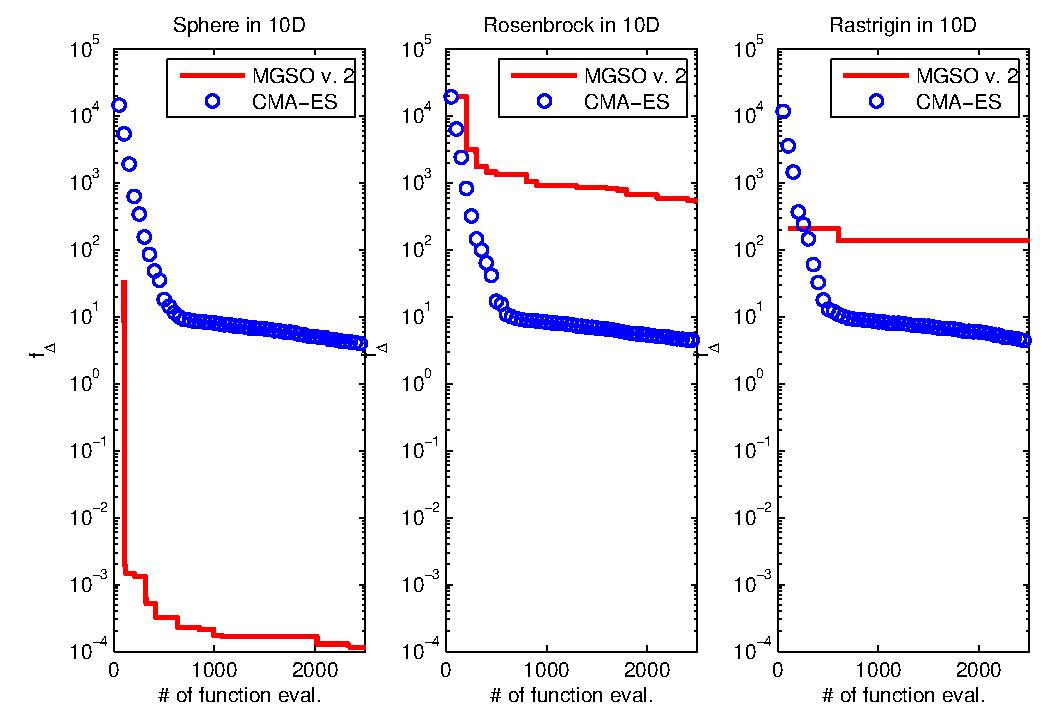
\includegraphics[width=\linewidth]{optim_10D_color}
  {\small
    % \caption{10-D. Medians of the best found function values gathered from 15 runs on different function instances of the three BBOB functions. The second version of MGSO is compared to CMA-ES.
    \caption{5-D. Medians of the best found function values gathered from 15 runs. The second version of MGSO is compared to CMA-ES.
  \label{fig:optim_10D}
  }
  }
\end{figure}

The MGSO scales nicely on the unimodal and symmetric sphere function. Both in 5D and 10D, a dramatically lower number of function evaluations is needed to reach threshold of the objective function values $f_{\Delta} = 10^{-4}$ than in the case of CMA-ES, see Fig.\,\ref{fig:optim_5D} and Fig.\,\ref{fig:optim_10D}. On the Rosenbrock function, however, the number of evaluations of MGSO needed to reach $f_{\Delta} = 10^{-2}$ is lower in 5D, but CMA-ES works better in 10D. The multimodal Rastrigin function with large number of local minima is not harder than the two other functions for CMA-ES, but it is not the case of the MGSO. Our algorithm is outperformed by CMA-ES in both 5D and 10D for that benchmark function.


\subsection{Conclusions and future work}

Our method shows promising results in terms of the number of true objective function evaluations in the initial phase of optimization. However, there are still many issues to solve. In general, we are planning to work on improving the final local optimization in the region of the optimum either by improving MGSO itself or combining it with some other method in the final phase. Further, fitting of the hyper-parameters of the GP model will be studied, since GPML implementation\footnote{\url{http://www.gaussianprocess.org/gpml/code/matlab/}}~\cite{rasmussen_gaussian_2010} being used is often not able to fit them to optimal values.

Future work should also test different initial sampling schemes, which affect the model quality and thus performance of the method and perform rigorous testing of the effects of input parameters, which were set by hand for our initial experiments. A comparison with the EGO method, which was not done due to a lack of a readily available implementation, will also be performed. 

The Model Guided Sampling Optimization was introduced in more detail. Several improvements of this algorithm were given and more experimental results than in the last brief work~\cite{bajer_model_2013} were provided. The experiments show that the proposed method can successfully compete with the state-of-the art continuous black-box optimization algorithm CMA-ES in lower dimensions and on unimodal symmetric functions.


% \noindent ==================
% 
% Evolutionary algorithms evolve in parallel a set of candidate solutions (a population) in multiple steps. Every iteration (in evolutionary context called generation) the candidate solutions (individuals) are evaluated with the objective function (so called fitness function). Then, some of these individuals are selected; the better ones are preferred. Finally, the selected individuals are modified or recombined between each other, a new population is created and a new generation starts again.
% 
% \paragraph{Surrogate Modelling.}
% Approximation of the fitness function with some regression model is a common cure for tasks when empirical objective function has to be used. These \textit{surrogate models} simulate behaviour of the original function while being much cheaper and much less time consuming to evaluate. As a surrogate model, any suitable regression model can be used~\cite{hosder2001polynomial,buche2005accelerating,ulmer2005model}.
% 
% In connection with evolutionary optimization, artificial neural networks of the type multilayer perceptrons \cite{jin2005neural} and networks with radial basis functions \cite{zhou2007combining,ong2004surrogate} have been particularly popular. The last mentioned kind of neural networks underlies also the model reported in this paper.





\subsection*{Acknowledgments}

This work was supported by 
the Czech Science Foundation (GA\v{C}R) grants \hbox{P202/11/1368} and \hbox{13-17187S}, 
the Grant Agency of the Charles University (GAUK) \hbox{278511/2011} grant and 
the Grant Agency of the Czech Technical University in Prague, grant No.~\hbox{SGS12/196/OHK3/3T/14}.


%
% ---- Bibliography ----
%
\bibliography{bajer2013itat}  % sigproc.bib is the name of the Bibliography in this case
\bibliographystyle{abbrv}

% %
% \begin{thebibliography}{5}
% %
% \bibitem {clar:eke}
% Clarke, F., Ekeland, I.:
% Nonlinear oscillations and
% boundary-value problems for Hamiltonian systems.
% Arch. Rat. Mech. Anal. {\bf 78} (1982) 315--333
% 
% \bibitem {clar:eke:2}
% Clarke, F., Ekeland, I.:
% Solutions p\'{e}riodiques, du
% p\'{e}riode donn\'{e}e, des \'{e}quations hamiltoniennes.
% Note CRAS Paris {\bf 287} (1978) 1013--1015
% 
% \bibitem {mich:tar}
% Michalek, R., Tarantello, G.:
% Subharmonic solutions with prescribed minimal
% period for nonautonomous Hamiltonian systems.
% J. Diff. Eq. {\bf 72} (1988) 28--55
% 
% \bibitem {tar}
% Tarantello, G.:
% Subharmonic solutions for Hamiltonian
% systems via a $\bbbz_{p}$ pseudoindex theory.
% Annali di Matematica Pura (to appear)
% 
% \bibitem {rab}
% Rabinowitz, P.:
% On subharmonic solutions of a Hamiltonian system.
% Comm. Pure Appl. Math. {\bf 33} (1980) 609--633
% 
% \end{thebibliography}

\end{document}
